\section{Arquitectura}
La arquitectura que dará solución a la situación problema será una arquitectura de tipo cliente-servidor, donde a continuación se describirá a detalle únicamente la arquitectura del cliente, en este caso la aplicación escrita en Python 3.7. El servidor no se describirá a detalle porque no es el objetivo de este documento, sin embargo en los apéndices se describen los endpoints y sus parámetros.

\subsection{Diagrama de clases}

A continuación se presenta el diagrama de clases creado en StarUML (ver referencias). Dicho diagrama se acopla a las convenciones para nombrar variables y métodos en Python, por lo que puede discrepar un poco con lo especificado por el estándar UML.

\begin{figure}[h!]
	\centering
	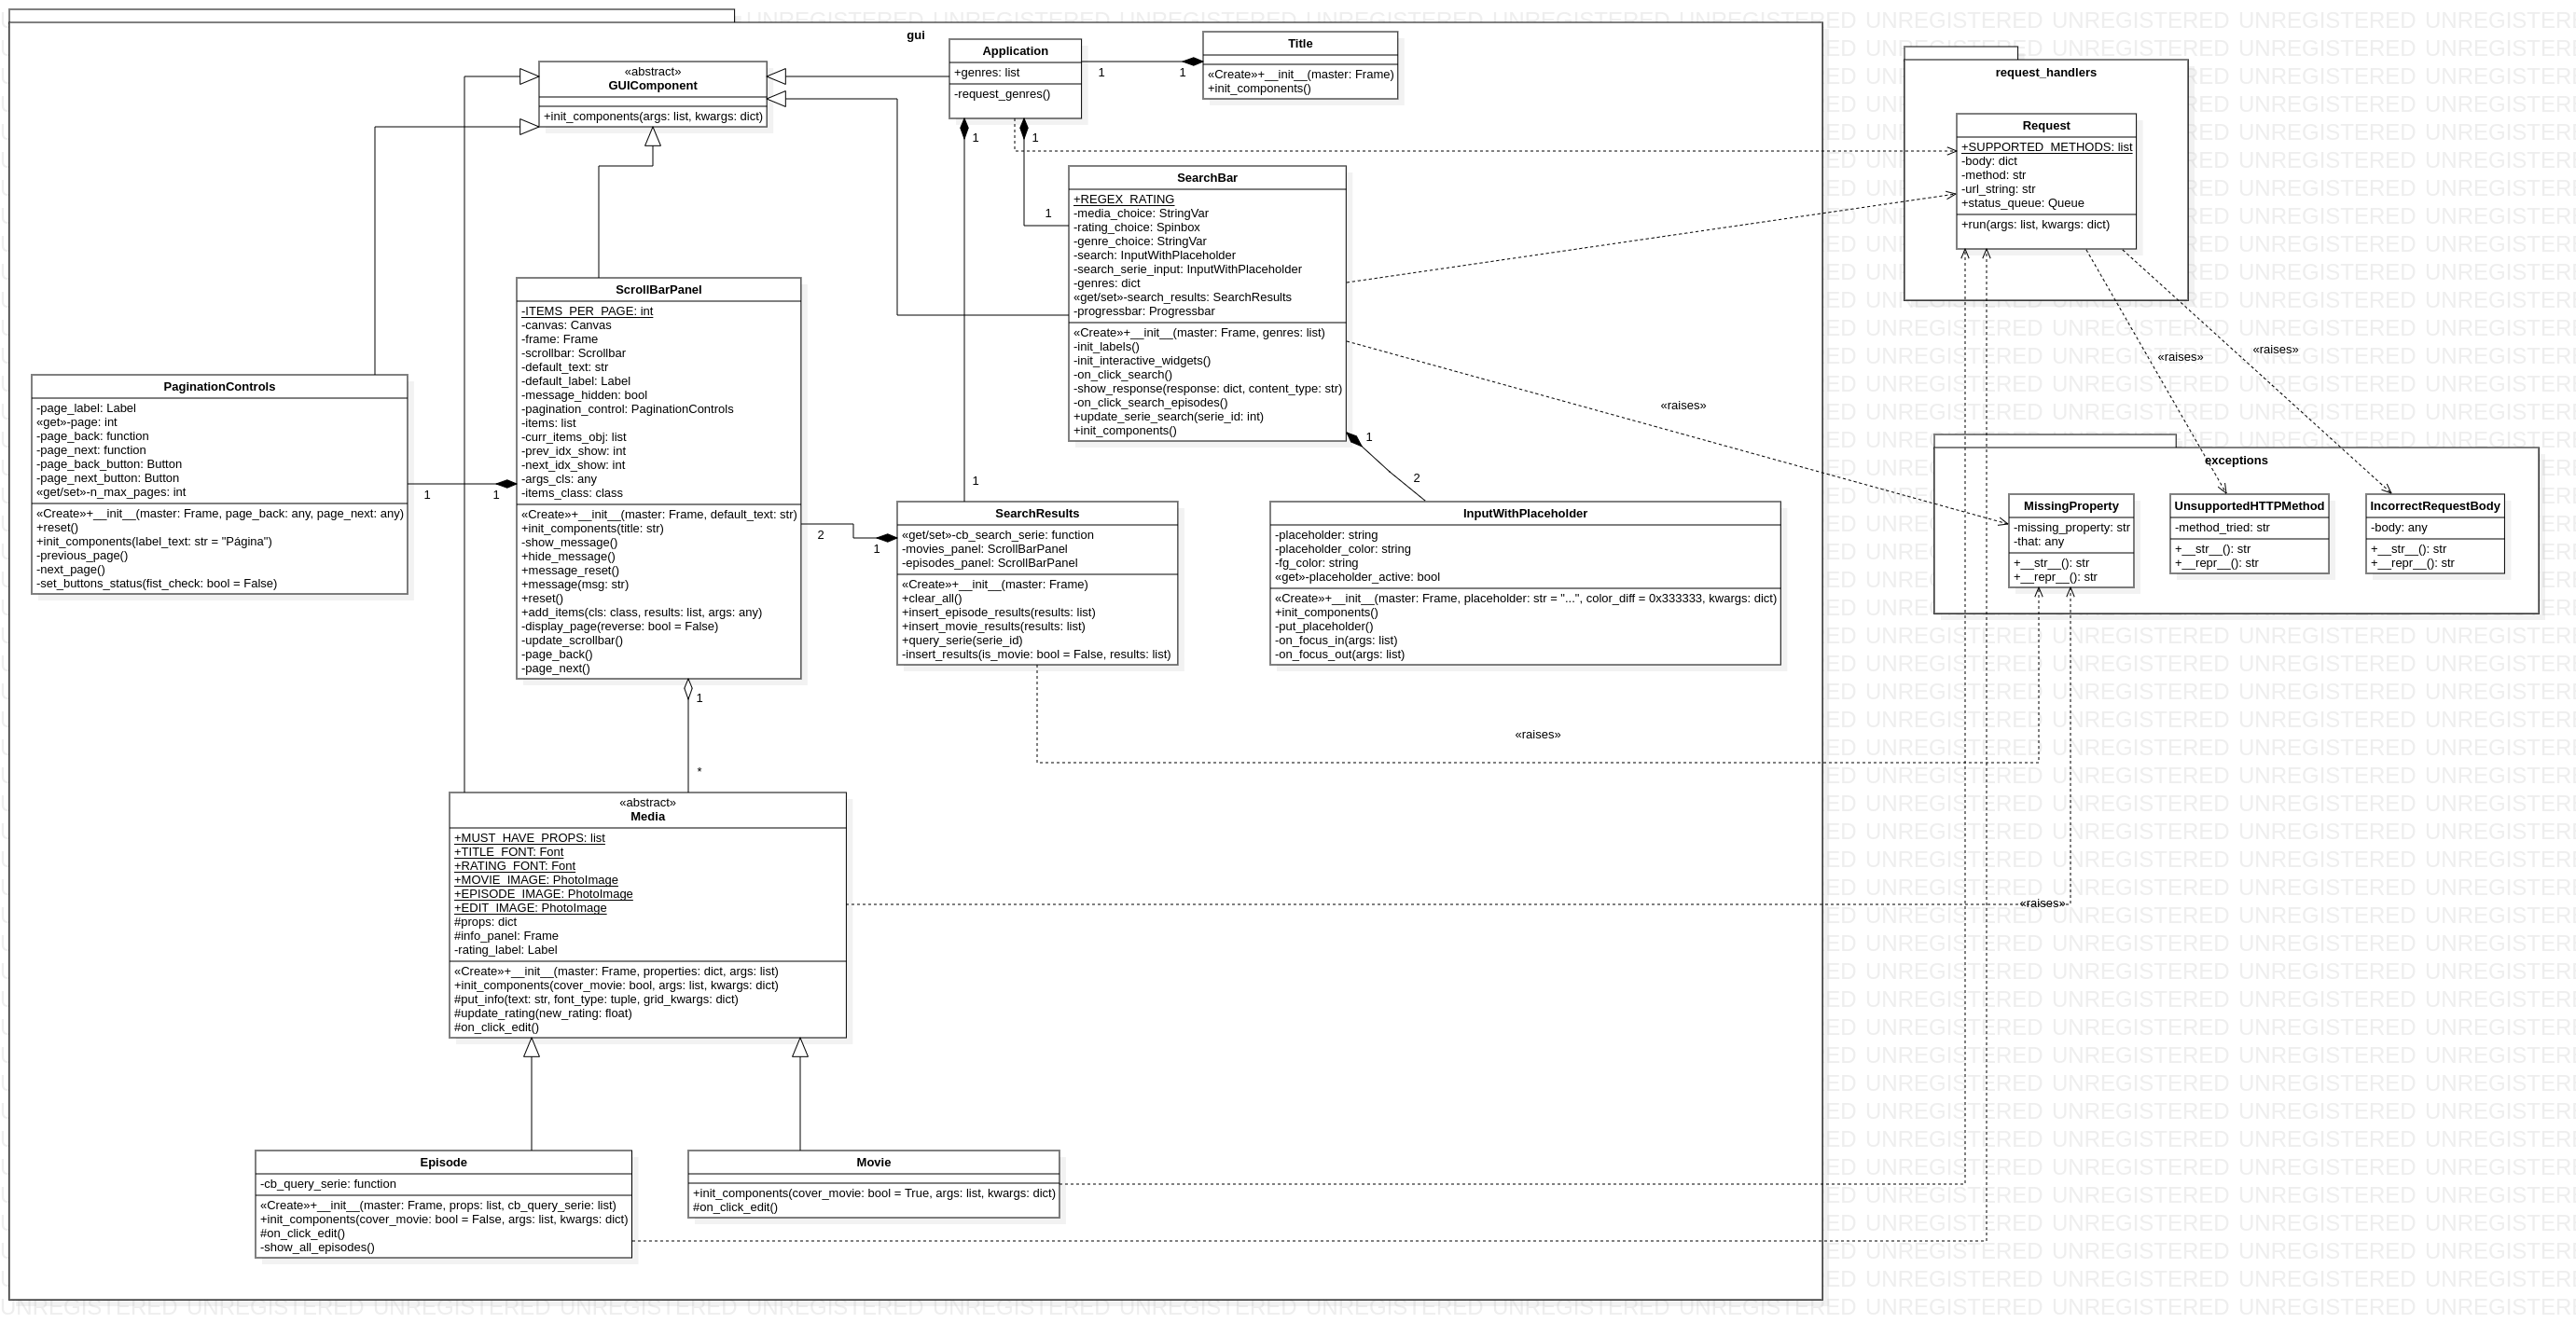
\includegraphics[width=1\linewidth]{class_diagram.png}
	\caption{Diagrama de clases para el front-end}
	\label{fig:class-diagram}
\end{figure}

\subsubsection{Paquete: gui}
Este paquete contiene todas las clases que construyen a la interfaz gráfica desde la cual el usuario interactúa con el servicio. La librería utilizada para crear la interfaz gráfica es tkinter (ver referencias), se eligió dicha librería porque ya está contenida en python 3 y no es necesario instalarla manualmente, además de que ya se contaba con conocimiento previo sobre cómo usarla.

Todas las clases de este paquete, excepto Episode, Movie, GUIComponent, InputWithPlaceholder y Application heredan directamente de la clase Frame proveída por tkinter, en el último caso, la clase Application hereda de la clase Tk también proveída por la misma librería. Todos aquellas clases utilizadas pero no programadas, es decir que las provee directamente Python 3 o una librería externa no se colocaron evidentemente en el diagrama.

\textbf{Clase GUIComponent}\newline
Esta realmente es una interfaz puesto que solo declara más no define el comportamiento de su método \mono{init\_components}, por lo que cada clase que implemente (herede) esta interfaz deberá implementar dicho método, además dichas clases pueden además sobreescribir o sobrecargar dicho método.
Este método difiere del constructor de una clase en que éste se encargará de instanciar los atributos de la clase que no sean componentes gráficos o que sean objetos parcialmente sencillos (como una lista vacía o valores por defecto), mientras que el método \mono{init\_components} se encargará de instanciar los componentes de la interfaz gráfica, así como de computar los valores de los atributos de la clase que sean más complejos (como llenar la lista vacía).

\textbf{Clase Application}\newline
Esta clase es la ventana principal y hereda de tkinter.Tk, sobreescribe el método \mono{init\_components} que se encargará de instanciar un objeto Request que hará una petición al back-end para obtener todos los géneros disponibles.
Esto se realiza porque los géneros son un parámetro de búsqueda para el usuario, por lo que la instancia de SearchBar de este objeto deberá tener conocimiento de los géneros para desplegarlos en un dropdown.
Además la cantidad de géneros es mucho menor a la cantidad de películas o episodios, por lo que cargar los géneros ocupa menos recursos que las otras entidades. Aunado a esto, la lista de géneros es indispensable para hacer la búsqueda (entre otros campos, que se pueden construir on-the-fly para ahorrar recursos, y se platicará sobre ello en la clase SearchBar).

\textbf{Clase Title}\newline
Si bien, la creación de esta clase no era muy necesaria, se decidió crear por simplicidad y legibilidad del código y por tener un diseño modular más sencillo. Dicha clase se encarga de crear los componentes que generan el título junto con el nombre del autor (Benjamín Antonio Velasco Guzmán A01750156).

\textbf{Clase SearchBar}\newline
Clase encargada de contener y desplegar los cuatro filtros para realizar una búsqueda:
\begin{itemize}
	\item Tipo de contenido: video, episodio o ambos
	\item Nombre del contenido: Caracteres con los que inicie el contenido que se desea buscar (e. g. "The D", si se desea buscar "The Dark Knight")
	\item Rating mínimo: El rating mínimo (números del 0 al 10 con saltos de 0.5) que debe tener el contenido que se desea buscar.
	\item Género: El género del contenido que se desea buscar.
\end{itemize}

Esta clase también es la encargada de manejar todos los eventos relacionados a la búsqueda, es decir se encarga de instanciar un objeto Request para realizar la petición de búsqueda en el back-end en cuanto se da click al botón de "Buscar", y con los resultados recibidos notifica al objeto SearchResults instanciado por Application para finalmente mostrar los resultados.

En esta clase también se lleva a cabo la validación de la entrada del usuario, específicamente del Rating mínimo, que es un campo de texto que potencialmente pueden recibir cualquier texto aunque sólo los números enteros o decimales con sólo un decimal son recibidos.

No se lleva a cabo la validación de otros campos porque no son campos que puedan recibir cualquier entrada, son dropdowns con valores válidos predefinidos.

\textbf{Clase InputWithPlaceholder}\newline
Extiende de tkinter.Entry, y se encarga de colocar un placeholder en el input simplemente por estética, esta clase no es lógicamente indispensable. Naturalmente esta clase maneja todos los eventos de focus in/out sobre el input para remover o colocar el placeholder, junto con el manejo de colores para diferenciar el placeholder del texto insertado.

\textbf{Clase SearchResults}\newline
Clase encargada de contener a dos paneles que contendrán a su vez los resultados de las películas y episodios resultantes (de ahí que se requieran dos paneles). Esta clase al igual que Title no tiene mucho funcionamiento pero es útil para separar lógicamente el código y servir de contenedor.

\textbf{SearchResults}\newline
Esta clase se encargará de instanciar a los objetos correspondientes de tipo Media (Episode o Movie), así como de destruir a los objetos instanciados cuando se cambie de página e instanciar los correspondientes de la nueva página. De la misma forma esta clase con ayuda de la clase PaginationControls se encargará de manejar los eventos de cambio de página.

\textbf{Clase PaginationControls}\newline
Clase encargada de contener un panel con los controles para la paginación y navegación sobre los resultados mostrados en un ScrollbarPanel. También se encarga de recibir los eventos de cambio de página, y ejecuta un callback previamente definido en la instancia del ScrollbarPanel que contiene a la instancia de esta clase para que se puedan mostrar resultados diferentes para cada página.

\textbf{Clase Media}\newline
Clase abstracta que contiene muchos métodos útiles para desplegar un resultado de una búsqueda independientemente de si es episodio o película, por ello contiene varios atributos con modificador de acceso tipo protected, así como otros métodos que pueden ser sobreescritos por sus clases hijas.
Dado que cualquier contenido, sea película o episodo contiene las siguientes propiedades:

\begin{itemize}
	\item rating
	\item duration
	\item name
\end{itemize}

Que son las que esta clase toma en cuenta para desplegar la información de cualquier tipo de contenido, si se desea agregar más contenido, éste deberá contenerse en la clase hija y para desplegarlo en la interfaz gráfica se proporciona el método \mono{put\_info}.

Naturalmente este diseño permite bastante la reutilización de código, así como la generalización de tipos.

\textbf{Episode}\newline
Clase que hereda de Media, se encarga de mostrar y contener todos los atributos exclusivos de un episodio:

\begin{itemize}
	\item ID de la serie a la cual pertenece el episodio
	\item Nombre de la serie a la cual pertenece el episodio
	\item Número de episodio
	\item Número de temporada a la cual pertenece el episodio
\end{itemize}

Sobreescribe el método \mono{on\_click\_edit} para editar el rating del episodio y enviar la petición al backend. Para ello crea una instancia de Request. Esto sucede claramente después de pedirle al usuario el nuevo rating para el episodio mediante un cuadro de diálogo que también tiene validación para sólo ingresar números flotantes entre 0 y 10.

De igual forma tiene su método propio \mono{show\_all\_episodes} para que al darle click al botón "Ver serie" se muestren todos los episodios de la serie. Evidentemente esta clase también crea y maneja el botón previamente mencionado

\textbf{Movie}\newline
Clase que hereda de Media, una película al tener los mismos atributos que Media, no existen muchas implementaciones o sobreescrituras de métodos, salvo el método \mono{on\_click\_edit} que crea una instancia de Request y envía una petición al back-end para actualizar el rating de la película. Esto sucede claramente después de pedirle al usuario el nuevo rating para el episodio mediante un cuadro de diálogo que también tiene validación para sólo ingresar números flotantes entre 0 y 10.

\subsubsection{Paquete: request\_handlers}
Este paquete, a pesar de solamente contener una clase se decidió separar por simplicidad y un mejor control de los archivos, además de que el uso de la única clase Request que contiene es de propósito general, se puede usar en alguna clase dentro del paquete gui o fuera.

\textbf{Clase Request}\newline
Clase que hereda de Thread, y se encarga de enviar peticiones HTTP al backend. Como se mencionó, esta clase intenta ser de propósito general por lo que el método de la petición, payload o body, ruta e incluso host y puerto son definidos por quien instancie un objeto de esta clase.

Al tener en cuenta que esta clase será usada dentro del paquete gui y mientras el hilo de ejecución principal esté principalmente ocupado por la interfaz gráfica, se decidió que esta clase heredara de Thread para evitar interferir y bloquear el hilo principal, por esta naturaleza de ejecución paralela también se utilizó mutex (mutual exclusion) para modificar el atributo status\_queue que contiene el último status reportado, de forma tal que quien use esta clase pueda saber el estatus de su petición mediante la obtención del primer valor en la queue (recordar que la cola o queue funciona con el principio FIFO (First In First Out), además de que python guardará la queue en heap, lo que hace posible que tanto Request como la clase que usa Request puedan acceder al mismo objeto)

Las anteriores consideraciones pudieron no haber sido tomadas en cuenta dados los bajos niveles de concurrencia y trabajo que puede llegar a tener la aplicación (de hecho, de todas formas se bloquea el hilo principal de la aplicación mientras se recibe la respuesta del back-end pues no es necesario por el momento que se ejecute estrictamente en otro hilo la petición), pero se decidió implementar por escalabilidad y buena práctica de ingeniería de software.

Por último, esta clase puede lanzar excepciones definidas en el paquete exceptions si el backend no soporta algún método (HTTPMethodUnsupported) o si el payload o body de la petición no es correcto (IncorrectBodyRequest)

\subsubsection{Paquete: exceptions}
Contiene las excepciones no estándar definidas por mí. Cabe recalcar que no son las únicas excepciones que puede lanzar algún método o función, de hecho en el paquete gui se lanzan excepciones predefinidas también.

\textbf{MissingProperty}\newline
Excepción útil cuando hace falta o tiene valor None algún atributo de la clase, usualmente esto se debe a una mala inicialización del objeto o debido a que no se invocó algún método que coloque valores correctos a los atributos de una clase (e. g. \mono{init\_components})

\textbf{UnsupportedHTTPMethod}\newline
Excepción estrictamente relacionada a la clase Request, pues este error es lanzado cuando se intenta realizar una petición al back-end con un método no soportado.

\textbf{IncorrectBodyRequest}\newline
Nuevamente, es una excepción estrictamente relacionada a la clase Request, pues este error es lanzado cuando se intenta enviar un payload o body que no sea \mono{dict} o herede de esta clase (la conversión y correcta codificación del objeto es manejada por el paquete requests)